\chapter{Background}
\label{chpt:background}

\section{Meta Pseudo-Labels}
Large models usually tend to overfit on 
small labeled datasets, and semi-supervised learning can help to mitigate this 
issue by leveraging the information contained in the unlabeled data.
However, to apply semi-supervised learning methods in practice, unlabeled data 
needs to carry useful information that is not already contained in the labeled 
dataset. This hypothesis can be formulated through three different assumptions: 
\emph{smoothness}, \emph{clusters}, and \emph{manifold} 
\cite{chapelle2010semi}.

In a more formal formulation, given $p(y|\bm{x}, D_L)$ as the probability 
distribution over the possible classes, given the input $x$ and the labeled 
dataset $D_L$, the goal is to estimate $p(y|\bm{x}, D_L, D_U)$, where $D_U$ is the 
unlabeled dataset. We can say that semi-supervised learning is effective only if 
$p(y|\bm{x}, D_L, D_U)$ is more accurate than $p(y|\bm{x}, D_L)$. If it is not 
the case, semi-supervised learning does not provide any additional benefit to 
the inference of the model, and it could even deteriorate the performance 
\cite{chapelle2010semi}.

\subsection{Smoothness Assumption}
\textbf{Assumption}: If two examples are close in the input space, then they 
have similar outputs (labels).

The smoothness assumption implies that slightly changing the input data should 
not drastically change the output. Therefore, also the model is supposed to 
predict similar outputs for similar inputs. This assumption is fundamental in 
the propagation of the labels on the unlabelled data from the prior knowledge.

In Figure \ref{fig:moon_cluster}, on the left, the smoothness assumption is 
illustrated with an example on the moon dataset. The smoothness assumption 
is satisfied because similar points, in terms of the distance, have the same 
output.

\subsection{Cluster Assumption}
\textbf{Assumption}: Data points are orgnaized in clusters, and points that 
belong to the same cluster are more likely to have the same label.

This assumption supports methods like clustering followed by label propagation, 
where each cluster receives a common label, potentially inferred from a few 
labeled examples within or near the cluster.
It does not imply that each class is related to a unique cluster. 
On the other hand, it means that it is not possible to have two different classes 
in the same cluster.
From this hypothesis, it is also derived the \emph{low-density separation} 
assumption, which imposes that the decision boundary should lie in low-density
regions between clusters.

In Figure \ref{fig:moon_cluster}, on the right, the cluster assumption is 
illustrated with 2D data points organized in clusters. Each cluster's point is 
more likely to have the same label.
\begin{figure}[h]
    \centering
    \begin{minipage}{0.5\textwidth}
        \centering
        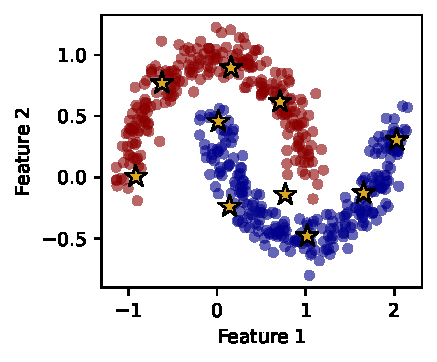
\includegraphics[height=5.5cm]{images/ssl/moon.pdf} % first figure
    \end{minipage}\hfill
    \begin{minipage}{0.44\textwidth}
        \centering
        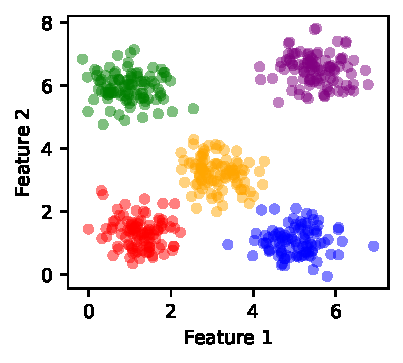
\includegraphics[height=5.5cm]{images/ssl/clusters.pdf} % second figure
    \end{minipage}
    \caption [Illustration of the smoothness and cluster assumptions.]
    {Smoothness and cluster assumptions. \textbf{Left}: The moon dataset representing smoothness between 
        data points of each class. \textbf{Right}: The cluster assumption 
        illustrated with a toy example.}
    \label{fig:moon_cluster}
    \end{figure}
\begin{figure}[h]
    \centering
    \begin{minipage}{0.4\textwidth}
        \centering
        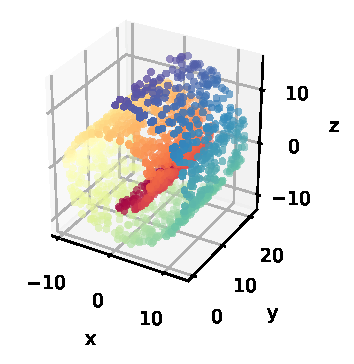
\includegraphics[height=5.5cm]{images/ssl/swiss_roll_3d.pdf} % first figure
    \end{minipage}\hfill
    \begin{minipage}{0.55\textwidth}
        \centering
        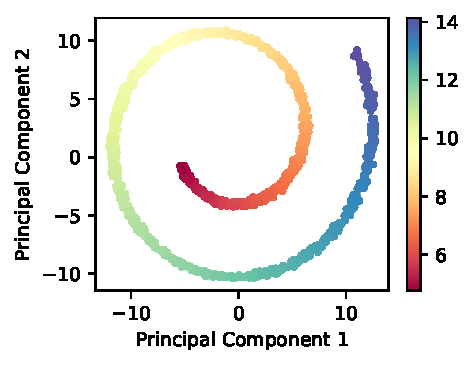
\includegraphics[height=5.5cm]{images/ssl/swiss_roll_pca.pdf} % second figure
    \end{minipage}
    \caption[Illustration of the manifold assumption.]
    {Illustration of the manifold assumption. 
        \textbf{Left}: Data points are distributed in a high-dimensional space. 
        \textbf{Right}: The data points lie on a lower-dimensional manifold.}
    \label{fig:swiss_roll}
\end{figure}

\subsection{Manifold Assumption}
\textbf{Assumption}: The data lies on a low-dimensional manifold embedded in a 
high-dimensional space.

This assumption is based on the idea that the data is not distributed uniformly 
in the input space, but it is concentrated on a lower-dimensional manifold.
It is fundamental to avoid problems related to the curse of dimensionality, 
which can lead to overfitting and poor generalization because of sparse data.

In Figure \ref{fig:swiss_roll}, the manifold assumption is illustrated with the 
Swiss roll dataset. The data points are distributed in a three-dimensional 
space, but they lie on a two-dimensional manifold. In general, the principal 
components analysis (PCA) can be used to reduce the dimensionality of the data, 
and in this specific case principal components are respectivlely the $x$ and $z$ 
axes.


\subsection{The Training Algorithm}
Classical pseudo-labeling methods usually train the teacher model on the labeled 
data and then they keep it fixed to predict the labels on the unlabeled data. 
The pseudo-labels are then used to train the student model, which is a copy of 
the teacher model. The student model is finally trained on the pseudo-labelled 
data.

On the other hand, on Meta Pseudo-Labels \cite{pham2021meta}, the teacher is 
trained along with the student model. In particular the student model is trained 
on the pseudo labels generated by the teacher model, and the teacher is trained 
on the performance of the student model on the labeled data. This process is 
repeated until the student model converges reaching a better performance 
with respect to the teacher. Therefore, the teacher model is updated to 
maximize the performance of the student.

In a more formal way, Pseudo Labels aims to optimize the student's 
loss function $CE(T(x_u, \theta_T), S(x_u, \theta_S))$, with the pseudo-labels 
generated from the teacher on the unlabeled data:
\begin{align}
    \theta_S^{PL} &= \arg \min_{\theta_S} \mathbb{E}_{x_u}\left[
        {CE(T(x_u, \theta_T), S(x_u, \theta_S))}\right] 
        \label{eq:pl_student_param}\\
        &:=
        \arg \min_{\theta_S} \mathcal{L}_u(\theta_T, \theta_S) \nonumber
\end{align}
where $T(x_u, \theta_T)$ is the pseudo target generated by the trained teacher 
model with its parameters $\theta_T$ already optimized and fixed. 
Therefore, the final goal of 
Pseudo Labels is to have a lower student loss with respect to the teacher on 
the labelled data:
\begin{align}
    \mathbb{E}_{x_l, y_l}\left[CE(y_l, S(x_l, \theta_S^{PL}))\right]
    &\leq
    \mathbb{E}_{x_l, y_l}\left[CE(y_l, T(x_l, \theta_T))\right]
    \qquad \Longleftrightarrow 
    \label{eq:pl_student_loss}\\
    \mathcal{L}_l(\theta_S^{PL})
    &\leq\
    \mathcal{L}_l(\theta_T) 
    \nonumber
\end{align}
Combining Equations (\ref{eq:pl_student_param}) and (\ref{eq:pl_student_loss}) 
it is possible to notice that the student loss $\mathcal{L}_l(\theta_S^{PL})$ 
depends on the teacher parameters $\theta_T$. Therefore, it could be possible 
get a better optimization of the teacher model to reduce the student loss. 
This is the main idea behind Meta Pseudo-Labels.
The final student loss $\mathcal{L}_l^*(\theta_S^{PL})$ will be the following:
\begin{align}
    \mathcal{L}^*_l(\theta_S^{PL*}) &= \min_{\theta_T} \mathcal{L}_l(\theta_S^{PL}(\theta_T))
    \label{eq:pl_student_loss_final} \\
    \text{where} \qquad \theta_S^{PL}(\theta_T) &= \arg\min_{\theta_S} \mathcal{L}_u(\theta_T, \theta_S)
    \nonumber
\end{align}
However, calculating the gradient $\nabla_{\theta_T}\theta^{PL}_S(\theta_T)$ 
is computationally expensive and complicated to get because it requires to 
unroll all the previous training of the student, given that $\theta_S^{PL}$ was updated 
multiple times with a combination of the fixed $\theta_T$.
To overcome this issue, Meta Pseudo-Labels uses a meta-learning approach to 
approximate  
the computation of $\theta_S^{PL}(\theta_T)$ to a single step:
\begin{align}
    \theta_S^{PL}(\theta_T) &\approx \theta_S - \eta_S \nabla_{\theta_S} \mathcal{L}_u(\theta_T, \theta_S)
    \label{eq:pl_student_update}
\end{align}
where $\eta_S$ is the learning rate used for training the student model.
In this way, the objective function to optimize the student introduced in 
Equation (\ref{eq:pl_student_loss_final}) can be approximated as follows:
\begin{align}
    \mathcal{L}^*_l(\theta_S^{PL}) &\approx \min_{\theta_T} \mathcal{L}_l(\theta_S - \eta_S \nabla_{\theta_S} \mathcal{L}_u(\theta_T, \theta_S))
    \label{eq:pl_student_loss_final_approx}
\end{align}
The final step that distinguishes Meta Pseudo-Labels from other pseudo-labeling 
algorithms is to not keep the teacher fixed during the training of the student. 
With the approximation introduced in Equation (\ref{eq:pl_student_update}), 
the objective function can be updated depending on the information provided only 
at the previous iteration.
Therefore, the teacher is trained along with the student.
The combined training can be summarized in the following steps:

\begin{itemize}
    \item \textbf{Student}: Sample a batch from unlabeled data $x_u$, get the 
    corresponding pseudo-labels $T(x_u, \theta_T)$, and update the parameters: 
    $\theta_S \leftarrow \theta_S - \eta_S \nabla_{\theta_S} \mathcal{L}_u(\theta_T, \theta_S)$.
    \item \textbf{Teacher}: Sample a batch from labeled data $(x_l, y_l)$ and 
    use the new student's parameters to optimize the objective function:
    $\theta_T \leftarrow \theta_T - \eta_T \nabla_{\theta_T} \mathcal{L}_l(\theta_S)$.
\end{itemize}


\section{The Vision Transformer}

Transformers, originally developed for natural language processing tasks, have 
revolutionized the way machines understand and generate text. 
This model architecture, introduced by Vaswani et al. in the paper 
"Attention is All You Need" \cite{attention_is_all_you_need} relies on a 
mechanism known as self-attention to 
process data sequences in parallel, significantly improving efficiency and 
scalability compared to prior methods that used recurrent layers.

Building on the success in NLP, the concept of transformers has been adapted 
for image recognition tasks, marking a significant departure from the 
conventional convolutional neural networks (CNNs) that have dominated the field 
for years. This adaptation was most notably realized in the Vision Transformer 
(ViT) model introduced by Dosovitskiy et al. \cite{vit}. Their research demonstrates how a 
pure transformer applied directly to sequences of image patches can perform at 
or above current state-of-the-art levels on major image recognition benchmarks 
like ImageNet.

This approach challenges the prevailing reliance on CNNs for image tasks, 
suggesting that transformers can equal or exceed CNN performance on benchmarks 
with sufficient training data and computational power. The implications of this 
finding are fundamental, indicating a potential shift towards more flexible and 
scalable models for not only image classification but potentially other computer 
vision tasks as well.
Moreover, it proves that the transformer's ability to handle 
spatial data can be as effective in visual tasks as it has been in 
processing text.

In their paper, "An Image is Worth 16x16 Words: Transformers for 
Image Recognition at Scale" \cite{vit} the authors propose a straightforward yet 
highly 
effective approach: an image is divided into fixed-size patches, these patches 
are linearly embedded, and positional embeddings are added to retain positional 
information. The resulting sequence of vectors is then fed into a standard 
transformer architecture, similar to that used for NLP tasks. The model is 
trained end-to-end for image classification tasks, leveraging extensive 
pre-training on large datasets followed by fine-tuning on targeted smaller 
datasets.

\begin{figure}
    \centering
    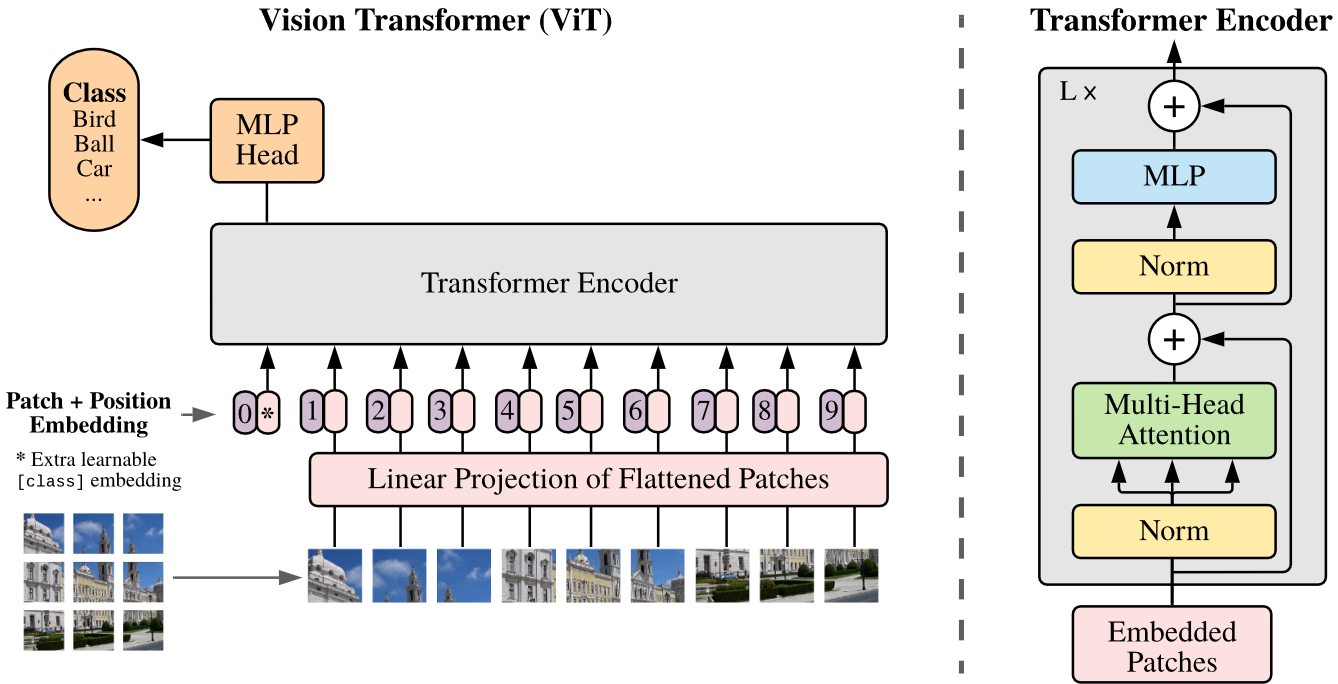
\includegraphics[width=0.8\textwidth]{images/vit/vit_scheme.png}
    \vspace*{0.3cm}
    \caption[The Vision Transformer architecture.]
    {The Vision Transformer architecture \cite{vit}. The input image is divided 
    into fixed-size patches, linearly embedded, and positional embeddings are 
    added. The resulting sequence of vectors is fed into the transformer encoder 
    architecture. On the top a feed-forward layer performs the classification.}
    \label{fig:vit_architecture}
\end{figure}

\subsection{Patch Embeddings}
Patch embedding is a key process that transforms raw image data into a format 
suitable for the transformer architecture. An image is first divided into small 
patches, which can be considered as sub-areas of the input image. 

Each patch is then flattened and projected into a higher-dimensional space 
through a linear transformation. This creates dense vector representations of 
the patches, like the word embedding process in NLP. 
Positional embeddings are added to these patch embeddings to preserve their 
spatial relationships, allowing the transformer to understand the layout of the 
image as it processes the sequence of embedded patches. 

This method adapts the transformer's powerful self-attention mechanisms to 
handle and interpret spatial relations of visual data.


\subsection{Self-Attention Mechanism}
The core of the transformer architecture is the self-attention mechanism, which 
allows the model to weigh the importance of different parts of the input data.
It is worth noting that the fundamental concept of self-attention does not 
require any trainable parameters. It is actually computed only through the 
embedded patches.

Considering a sequence of embedded patches $\{\boldsymbol{x_1, x_2, ..., x_t}\}$ 
as input, the self-attention is a sequence-to-sequence operation that outputs
$\{\boldsymbol{y_1, y_2, ..., y_t}\}$. The goal is to have each output vector 
$\boldsymbol{y_i}$ that represents a similarity between the $i$-th 
patch and all the input sequence of patches. In particular it can be described by a  
weighted sum of the input sequence
\begin{equation}
\boldsymbol{y_i} = \sum_{j=1}^{t} w_{ij} \boldsymbol{x_j}
\label{eq:self_attention_output}
\end{equation}
where $\boldsymbol{w_i}:=\{w_{ij}\}_{j=1}^t$ is the set of weights that describes the importance 
of each input vector for the $i$-th one. 
Therefore each $i$-th vector has a different set of weights with respect to 
the others.

The simplest way to compute the similarity is to use the dot-product between the 
input vectors $w'_{ij} = \boldsymbol{x_i^T x_j}$. Moreover, to guarantee them to have a limited 
range in $(0, 1)$ and to sum up to $1$, the softmax function is applied:
\begin{equation}
    w_{ij} = \boldsymbol{\sigma}(\boldsymbol{w'_i})_j = 
    \frac{e^{w_{ij}}}{\sum_{j} e^{w_{ij}}}
    \label{eq:attention_weights}
\end{equation}
From Equation (\ref{eq:attention_weights}) it is possible to notice that the 
weights depend only on the input vectors, and they are computed independently. 
That means that the self-attention mechanism is a parallel operation that does 
not consider the order of the input sequence. If the input sequence order is 
changed then the output sequence will change the order as well, keeping the 
same similarity results.

\subsection{Queries, Keys and Values}
In the self-attention task, each input vector $\boldsymbol{x_i}$ plays three 
different roles:
\begin{itemize}
    \item \textbf{Query}: $\boldsymbol{x_i}$ is used to compute the similarity to all the other 
    vectors in order to calculate $y_i$.
    \item \textbf{Key}: $\boldsymbol{x_i}$ is used to compute the similarity of 
    all the other vectors with respect to itself, in order to calculate all the 
    other outputs.
    \item \textbf{Value}: $\boldsymbol{x_i}$ is used to compute the weighted sum 
    of the input vectors, given the weights already computed.
\end{itemize}
This method introduces some controllable parameters that can be learned during 
the training to accomplish the respective tasks. In particular, the matrices 
are $\boldsymbol{W_q}, \boldsymbol{W_k}, \boldsymbol{W_v}$ and they all have 
dimesion $(q_k, q_k)$, given $q_k$ the embedding dimension of patches.
Equations (\ref{eq:self_attention_output}) and (\ref{eq:attention_weights}) can 
be rewritten as follows:
\begin{equation}
\begin{cases}
    w_{ij} = \boldsymbol{\sigma}(\boldsymbol{K^T q_i})_j \\
    \boldsymbol{y_i} = \sum_j w_{ij} \boldsymbol{v_j}
\end{cases}
\qquad
\text{where}
\quad
\begin{cases}
    \boldsymbol{q_i} = \boldsymbol{W_q x_i} \\
    \boldsymbol{K} = \boldsymbol{W_k X} \\
    \boldsymbol{v_j} = \boldsymbol{W_v x_j} \\
    \boldsymbol{X} = (\boldsymbol{x_1}, ..., \boldsymbol{x_t})
\end{cases}
\label{eq:self_attention_qkv}
\end{equation}
It is worthwile ntoicing that it is easier to consider the queries and values 
vectors, and the keys matrix. That is because the query is referred a specific 
input vector that is used to compute the similarity with all the others. 
The value is still directly related to the input vector used to compute the 
weighted sum. On the other hand, the keys are related to all the input vectors. 
Therefore, multiplying a query with the keys matrix will give all the similarities 
for the selected vector.

Adding trainable parameters to the self-attention mechanism allows to figure out 
the importance of all the sub-areas of the input image, depending on the bias we 
use to label the dataset. Then it is possible to use the attention mask, to 
highlight the importance of some specific areas of the image.

Finally, dot products between rows of $\boldsymbol{K^T}$ and 
$\boldsymbol{q_i}$ typically grow with the dimension of the embedding, 
and it can lead to instabilities in terms of gradients during the learning 
process. Therefore it is common to normalize the dot product by the square root 
of the embedding dimension $\sqrt{d_k}$, considering that it is also the 
grow rate of the Euclidean distance of the input vectors.

In a more general matrix form, Equation (\ref{eq:self_attention_qkv}) with the 
normalization can be 
described as follows:
\begin{equation}
Y = \boldsymbol{\sigma}\left(\boldsymbol{\frac{K^T Q}{\sqrt{d_k}}}\right) V\\
\qquad
\text{where}
\quad
\begin{cases}
    \boldsymbol{Q} = \boldsymbol{W_q X} \\
    \boldsymbol{K} = \boldsymbol{W_k X} \\
    \boldsymbol{V} = \boldsymbol{W_v X} \\
    \boldsymbol{X} = (\boldsymbol{x_1}, ..., \boldsymbol{x_t})
\end{cases}
\label{eq:self_attention_qkv_matrix}
\end{equation}
In Equation (\ref{eq:self_attention_qkv_matrix}) the softmax function 
$\boldsymbol{\sigma}$ is applied to the rows of its argument.


\subsection{Multi-Head Self-Attention Mechanism}
In an image each patch can have different relations with the others, depending 
on the context. Therefore, using only one self-attention mechanism would sum all 
the information together, limiting the ability to capture the scene context. 
To overcome this issue, the multi-head self-attention mechanism is introduced.
It is a parallel operation based on the single self-attention mechanism, which 
introduces multiple weight matrices $\boldsymbol{W_q^r, W_k^r, W_v^r}$, also 
called \emph{attention heads}.

It is also possible to keep the same number of parameters of the single 
self-attention mechanism in an efficient way. The main idea is to project queries, 
keys and values to a lower-dimensional space according to the number of heads.
In particular, given $h$ the number of attention heads, $d_k$ the embedding 
dimension of the patches, we can use a transformation matrix 
$\boldsymbol{T^r}$ of dimension $\left(d_k, d_k/h\right)$.
Therefore, the total number of parameters for
the single-head and multi-head self-attentions will be:
\begin{align*}
    \text{\#params SHA} &= 3 \cdot d_k^2 \\
    \text{\#params MHA} &= 3 \cdot h \cdot d_k \cdot\frac{d_k}{h} = 3 \cdot d_k^2
\end{align*}
\begin{figure}[htbp]
    \centering
    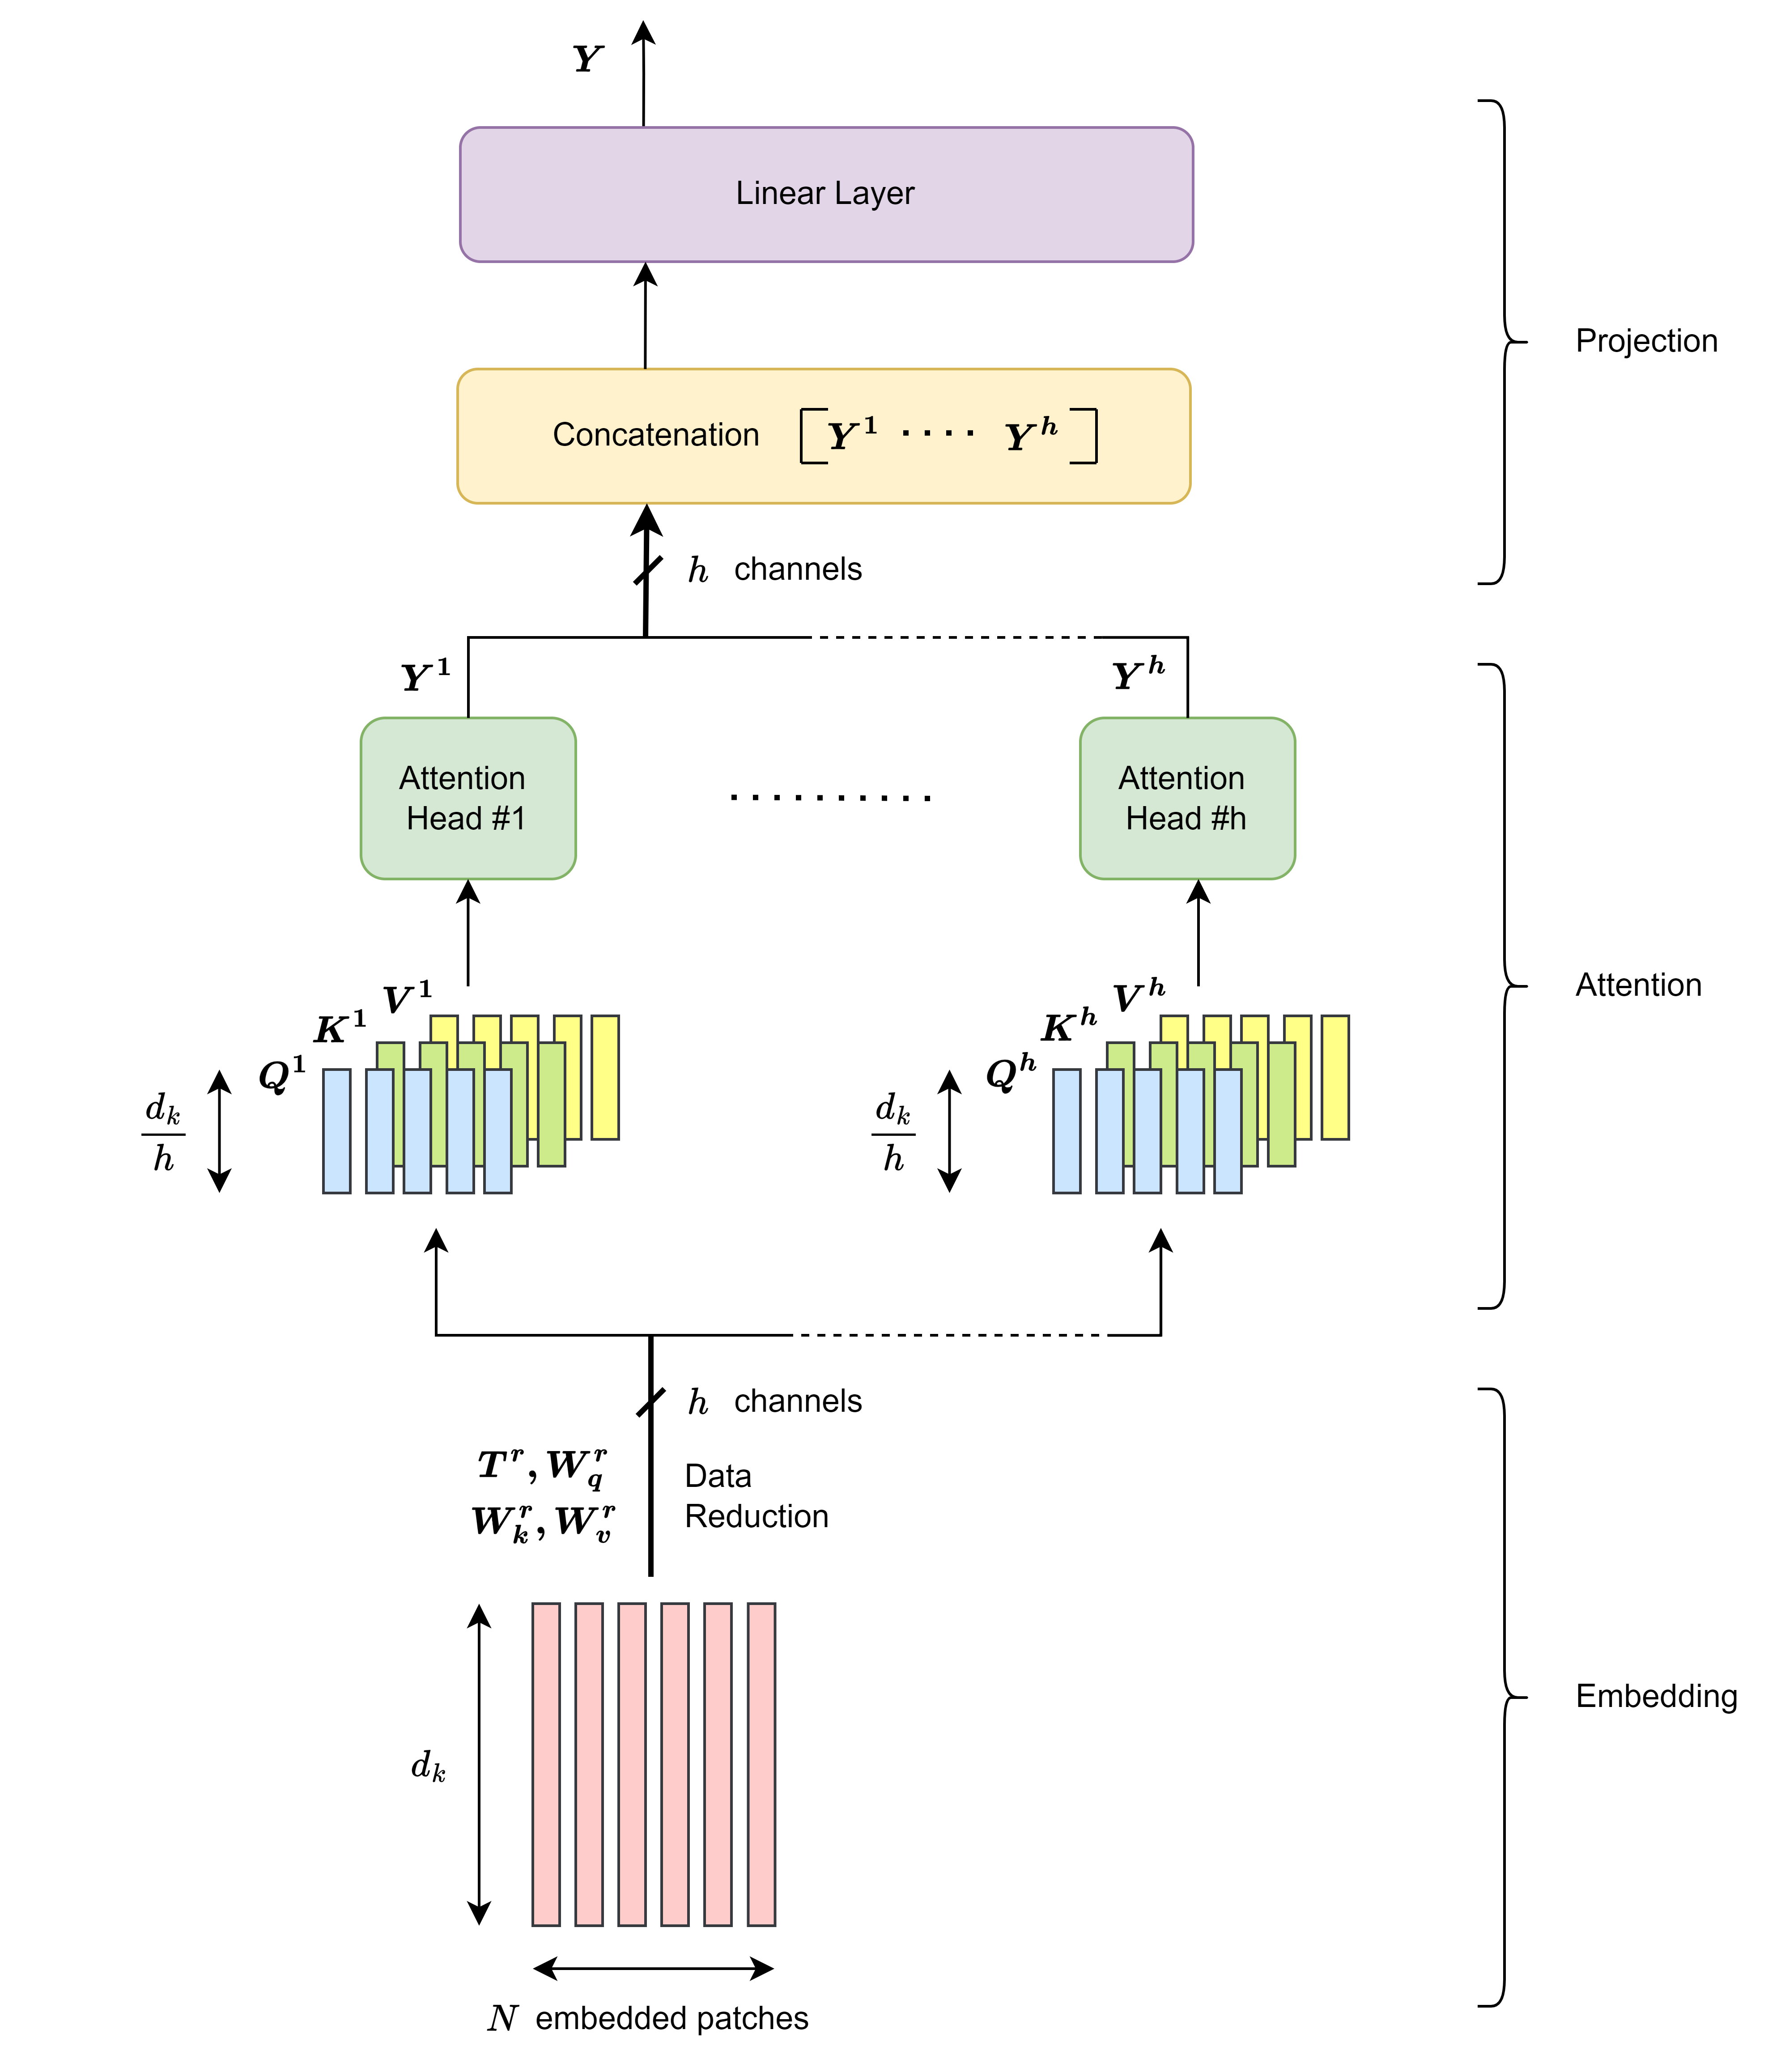
\includegraphics[width=\textwidth]{images/vit/multi_head_attention_scheme.png}
    \caption[Multi-head self-attention mechanism.]
    {Multi-head self-attention mechanism schematically represented with 
    the main blocks: patch embeddings, dimension reduction, attention heads, 
    data concatenation, and final linear transformation.}
    \label{fig:multi_head_attention}
\end{figure}
In Figure \ref{fig:multi_head_attention} the multi-head self-attention mechanism 
is schematically represented, and data flow is from the bottom to the top. 
The input patches are first embedded and projected to a lower-dimensional space. 
Therefore we get queries, keys and values for each attention head. 
The self-attention mechanism is applied to each head, and the outputs are 
concatenated together. In this way we augment the information of the spatial 
relation of each patch. Finally, a linear transformation is applied to get 
the final output of the multi-head self-attention mechanism, which describe the 
attention of each patch with respect to all the others.

To avoid any misunderstanding on the generation of the queries, keys, values and 
on the concatenation, data is represented through channels, where each channel is 
related to a specific attention head and it is independent from the others.

It is also worth noticing that the transformer architecture leverages on residual 
connections and layer normalization to stabilize the training process, avoiding 
the vanishing gradient problem. The residual connections are used to sum the 
output of the multi-head self-attention mechanism with the embedded patches, 
and the layer normalization is applied to the sum.

\subsection{Classification Transformer}
If the final task is a classification of the input image, it is necessary 
to have a feed-forward layer on the top of the transformer encoder, as shown in 
Figure \ref{fig:vit_architecture}.
Therefore, the final output will depend on the relative relation of the patches 
and their absolute location in the image.


\section{Traditional Computer Vision Techniques}
In this section we refer to some methods that have been used for a long time 
in computer vision tasks, even before the deep learning era. These methods 
are still used in some specific tasks, usually related to multiple view geometry.
In particular, the following methods are described: the \ac{sift} \cite{lowe_sift}, 
the Random Sample Consensus (RANSAC) \cite{ransac}, and the optimization 
algorithm to estimate the homography between two images.

\subsection{Scale Invariant Feature Transform (SIFT)}
The \ac{sift} algorithm is a method to detect and describe local features in 
images. It was introduced by David Lowe in 2004 \cite{lowe_sift}, and it is 
still used in computer vision tasks thanks to its robustness to changes in 
illumination, rotation, and scale. However, being computationally expensive, 
it is difficult to integrate it in real-time applications. Therefore other 
versions of the algorithm have been developed, like \ac{surf} \cite{surf} and
\ac{asift} \cite{asift}. These algorithms have also been implemented in 
computer vision libraries, like OpenCV, to leverage the power of parallel 
computing of GPUs.

The \ac{sift} algorithm is based on the following steps: scale-space peak
selection, keypoints detection, and assignment of descriptors to the keypoints.

\subsubsection*{Scale-Space Peak Selection}
To make the algorithm robust and scale-invariant, the first step is to analyze 
the image at different scales, applying a Gaussian filter with different 
standard deviations. Given an image $I(x, y)$, the scale-space representation 
is defined as: 
\begin{equation}
    L(x, y, \sigma) = G(x, y, \sigma) * I(x, y)
    \label{eq:scale_space}
\end{equation}
where $G(x, y, \sigma)$ is the Gaussian kernel with standard deviation $\sigma$.
The scale-space representation is computed for different values of $\sigma$, and 
the process is repeated for different octaves of the image. An octave is 
a set of images, each one with a resolution half of the previous one. The number 
of images for each octave is not standard, and it depends on the resolution 
of the original image.

The scale-space representation is used to detect the local maxima and minima 
of the difference of Gaussian (DoG) function. The DoG function is computed as 
the difference between two consecutive images of the same octave (let's say 
they have standard deviations $\sigma$ and $k\sigma$):
\begin{equation}
    D(x, y, \sigma) = L(x, y, k\sigma) - L(x, y, \sigma)
    \label{eq:dog}
\end{equation}
The local maxima and minima of the DoG function are detected by comparing each 
pixel with its eight neighbors in the same image and the nine neighbors in the 
previous and next images (26 in total). If the pixel is a local maxima or minima, it is 
considered a keypoint. To be a maxima or minima, the candidate pixel must be 
greater or smaller than all the neighbors, respectively.

\subsubsection*{Keypoints Localization}
The scale-space peak selection produces many keypoints, but not all of them are 
stable under changes in illumination, rotation, and scale. Therefore, the 
keypoints are filtered by applying the Taylor expansion to the DoG function 
for each candidate keypoint. The Taylor expansion is used to estimate 
the actual maxima or minima of the DoG function, approximated by the 
second-order derivative of the function with respect to the selected keypoint.

Considering the DoG function $D$ related to a keypoint, and an offset 
along all the dimensions
$\boldsymbol{x} = (dx, dy, d\sigma)^T$, 
to find accurate location of the selected keypoint a second-order Taylor expansion 
is computed as follows:
\begin{equation}
    D(\boldsymbol{x}) = D + \frac{\partial D}{\partial \boldsymbol{x}}^T \boldsymbol{x} + 
    \frac{1}{2} \boldsymbol{x}^T \frac{\partial^2 D}{\partial \boldsymbol{x}^2} \boldsymbol{x}
    \label{eq:taylor_expansion}
\end{equation}
Minima, or maxima, $\boldsymbol{\hat{x}}$ is detected by solving the equation:
\begin{equation}
    \boldsymbol{\hat{x}} = \arg \min_{\boldsymbol{x}} D(\boldsymbol{x})
    = \arg \{ \nabla_{\boldsymbol{x}} D(\boldsymbol{x}) = \boldsymbol{0} \}
\end{equation}

Keypoints with low intensity are filtered out, depending on a threshold. Therefore, 
the more accurate keypoint $\boldsymbol{\hat{x}}$ is discarded if:
\begin{equation}
    D(\boldsymbol{\hat{x}}) < \text{threshold}
\label{eq:contrast_threshold}
\end{equation}

To remove the keypoints that are located on edges, on the other hand, the ratio 
between the principal curvatures of the DoG function is computed. 
If the ration is greater than a threshold, it means that there is a high variation 
of intensity on one direction with respect to the other (typical of an edge). 
Otherwise the keypoint corresponds to a corner and it is kept.
Principal curvatures are given by the eigenvalues $\lambda_1$ and $\lambda_2$
of the Hessian matrix of the 
DoG function, and the ratio is computed as follows:

\begin{equation}
    \frac{\text{Tr}(H)^2}{\text{Det}(H)} = \frac{(r+1)^2}{r} < \text{threshold}
    \qquad
    \text{where:} \quad r = \frac{\lambda_1}{\lambda_2}
    \label{eq:edge_threshold}
\end{equation}
It is possible to notice that the evaluation function in Equation 
(\ref{eq:edge_threshold}) has a minimum when the two eigenvalues are equal, 
and it grows when the ratio between the two eigenvalues increases.

\subsubsection*{Keypoint Orientation}
To make the keypoints invariant to rotation of the image, the orientation with 
respect to the neighbor pixels is computed. The orientation is computed through 
two terms, the magnitude and the orientation of the gradient of the 
correspondent DoG function:
\begin{align*}
    m(x, y) &= \sqrt{\left[D(x+1, y) - D(x-1, y)\right]^2 + \left[D(x, y+1) - D(x, y-1)\right]^2} \\
    \theta(x, y) &= \arctan\left(\frac{D(x, y+1) - D(x, y-1)}{D(x+1, y) - D(x-1, y)}\right)
\end{align*}
The angle $\theta$ is computed in the range $[0, 2\pi]$, and it is quantized 
in a histogram with 36 bins. The assigned orientation consists of the peak of 
the histogram, and all the other peaks that are greater than 80\% of the maximum.

\subsubsection*{Keypoint Descriptor}
After having assigned the orientation to the keypoints, the final step is to 
assign a unique descriptor to each keypoint. 
A grid of 16x16 pixels is considered around the keypoint, and it goruped into 
4x4 macro-areas. For each macro-area, the gradient magnitude and orientation 
are computed, and they are grouped into 8 bins. Therefore, the descriptor is 
a 128-dimensional vector (4x4x8).

To make the descriptor invariant to rotation, the orientation of the keypoint 
is subtracted from each gradient orientation.
Moreover, to make the descriptor invariant to illumination changes, each 
magnitude is truncated to a maximum thrashold, and then normalized.

\subsubsection*{Matching Keypoints}
To match similar keypoints in two different images, the Euclidean distance 
between the descriptors can be computed. However, considering a descriptor, 
there could be more than one similar match on the other image (i.e. the second 
best match could be close to the best). To overcome this issue, the ratio between 
the best and the second best match is computed. If the ratio is less than a 
threshold, the match is considered valid.

\subsection{Projective Transformation}
A homography is the transformation between two planes under perspective projection.
This means that a planar object in transformed by a homogeraphy into its image 
sensor.
However, the transformation can also be seen between two cameras, if all points 
in the Euclidean space lie on the same plane.

In Figure \ref{fig:homography_scheme} the homography transformation between two 
camera planes is represented. Two cameras, with their own system of coordinates, 
are pointing to the same plane. All points in the Euclidean space lie on the 
same plane, and they are projected on the two cameras' planes. The homography 
matrix $\boldsymbol{H}$ is the transformation of the projected points between 
the two camera planes.

Considering a general point $P_i \in \mathbb{R}^{3}$ in the Euclidean space, 
lying on a plane, and its correspondent projections on the two cameras' planes
$\boldsymbol{p_i}, \boldsymbol{p_i'} \in \mathbb{R}^{2}$.
Without focusing on a specific point, and without loss of generality, projection 
can be described by the following equation:
\begin{align}
    \boldsymbol{\tilde{p}} &\sim \boldsymbol{H} \boldsymbol{\tilde{p}'} && \boldsymbol{H} \in \mathbb{R}^{3 \times 3}, 
    \label{eq:homography}\\
    & && \boldsymbol{\tilde{p}}, \boldsymbol{\tilde{p}'} \in \mathbb{P}^{2}\nonumber
\end{align}
where $\boldsymbol{\tilde{p}}$ and $\boldsymbol{\tilde{p}'}$ are homogeneous 
coordinates of the points $\boldsymbol{p}$ and $\boldsymbol{p'}$ in the 2D
projective space $\mathbb{P}^{2}$. It is worth to notice that $\boldsymbol{H}$ 
is the homography matrix, and it is defined up to a scale factor. Therefore, to 
fully define it, at least four correspondent points are required.
Considering homogeneous coordinates of the points, Equation (\ref{eq:homography}) 
can be rewritten as follows:
\begin{equation}
    \begin{bmatrix}
        x \\
        y \\
        1
    \end{bmatrix}
    =
    \begin{bmatrix}
        h_{11} & h_{12} & h_{13} \\
        h_{21} & h_{22} & h_{23} \\
        h_{31} & h_{32} & h_{33} \\
    \end{bmatrix}
    \begin{bmatrix}
        x' \\
        y' \\
        1
    \end{bmatrix}
    \label{eq:homography_matrix}
\end{equation}
\begin{figure}
    \centering
    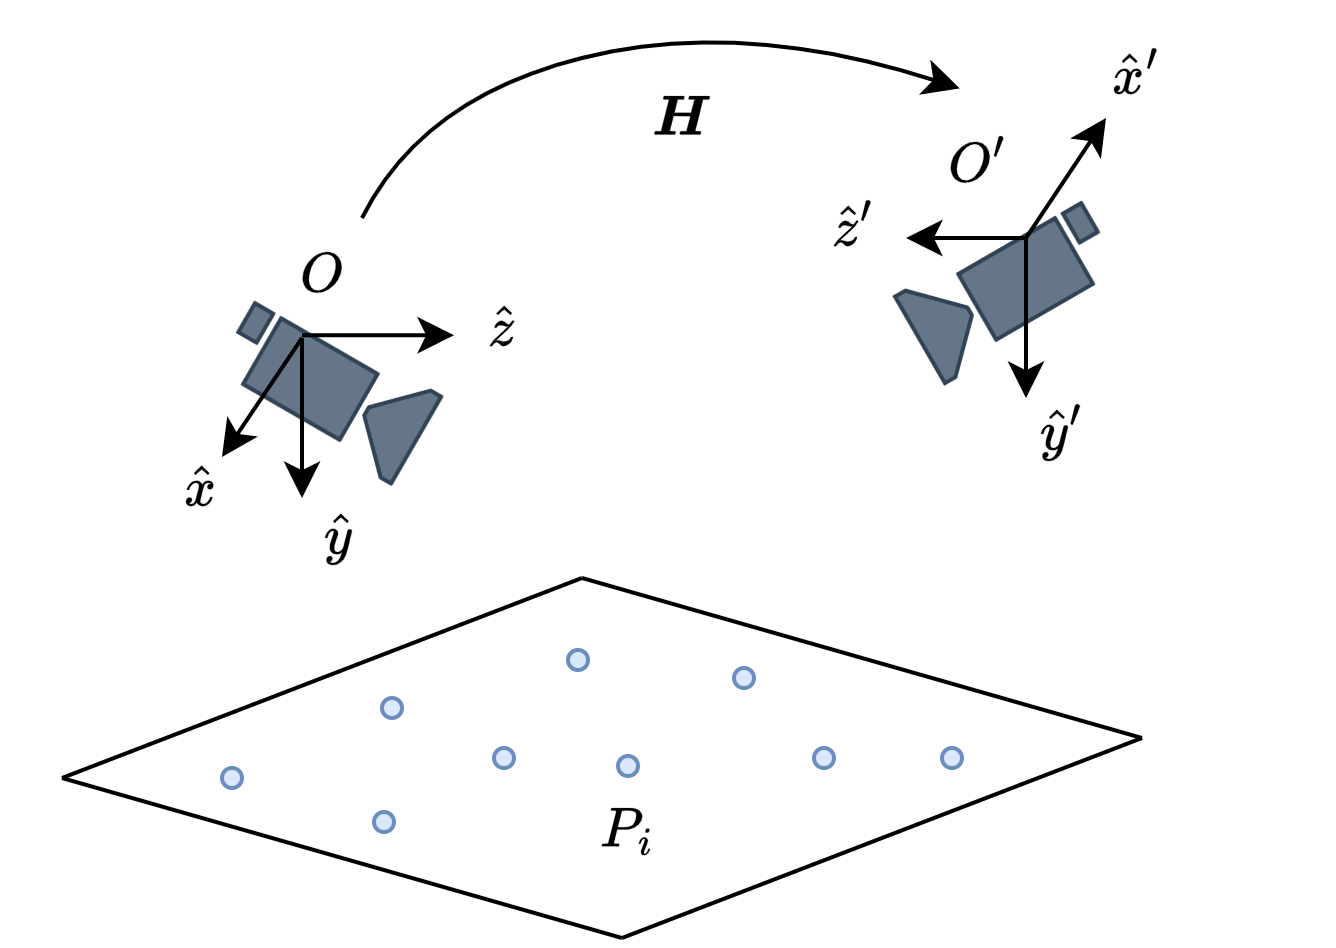
\includegraphics[width=0.6\textwidth]{images/dreyeve/homography.png}
    \vspace{0.2cm}
    \caption[Homography scheme.]
    {Homography between two planes. The transformation matrix defines the 
    projection between the camera planes. All points in the Euclidean space 
    lie on the same plane.}
    \label{fig:homography_scheme}
\end{figure}

\subsubsection*{Homography Estimation}
Given the $i$-th correspondance between two images, defined by the set 
$\{(x_i, y_i), (x_i', y_i')\}$, constraints described in Equation \ref{eq:homography_matrix}
are:
\begin{align}
&\begin{cases}
    x_i' = h_{11} x_i + h_{12} y_i + h_{13} \\
    y_i' = h_{21} x_i + h_{22} y_i + h_{23} \\
    1 = h_{31} x_i + h_{32} y_i + h_{33}
\end{cases}
\qquad \Longleftrightarrow \nonumber\\[0.2cm]
&\begin{cases}
    x_i' \left(h_{31} x_i + h_{32} y_i + h_{33}\right) = h_{11} x_i + h_{12} y_i + h_{13} \\
    y_i' \left(h_{31} x_i + h_{32} y_i + h_{33}\right) = h_{21} x_i + h_{22} y_i + h_{23}
    \label{eq:homography_constraints}
\end{cases}
\end{align}
In a matrix form, rearranging the terms to explicit terms of the homography matrix,
Equation (\ref{eq:homography_constraints}) can be written as:
\begin{equation}
    \begin{bmatrix}
        x_i & y_i & 1 & 0 & 0 & 0 & -x_i'x_i & -x_i'y_i \\
        0 & 0 & 0 & x_i & y_i & 1 & -y_i'x_i & -y_i'y_i
    \end{bmatrix}
    \begin{bmatrix}
        h_{11} \\
        \vdots \\
        h_{33}
    \end{bmatrix}
    =
    \begin{bmatrix}
        x_i' \\
        y_i'
    \end{bmatrix}
    \label{eq:homography_matrix_constraints}
\end{equation}
Considering now a general case with $n$ correspondences the problem to solve 
becomes in the form:
\begin{equation}
\begin{bmatrix}
    x_1 & y_1 & 1 & 0 & 0 & 0 & -x_1'x_1 & -x_1'y_1 & -x_1'\\
    0 & 0 & 0 & x_1 & y_1 & 1 & -y_1'x_1 & -y_1'y_1 & -y_1'\\
    \vdots & \vdots & \vdots & \vdots & \vdots & \vdots & \vdots & \vdots & \vdots \\
    x_n & y_n & 1 & 0 & 0 & 0 & -x_n'x_n & -x_n'y_n & -x_n'\\
    0 & 0 & 0 & x_n & y_n & 1 & -y_n'x_n & -y_n'y_n & -y_n'
\end{bmatrix}
\begin{bmatrix}
    h_{11} \\
    \vdots \\
    h_{33}
\end{bmatrix}
=
\boldsymbol{0}
\label{eq:homography_matrix_constraints_general}
\end{equation}
Equation (\ref{eq:homography_matrix_constraints_general}) is in the form of 
$\boldsymbol{Ah} = \boldsymbol{0}$, where $\boldsymbol{A} \in \mathbb{R}^{3x3}$
and $\boldsymbol{h} \in \mathbb{R}^{9}$.
When the number of correspondences is greater than 4, the system is overdetermined, 
and the homography matrix can be estimated by solving the least squares problem:
\begin{equation}
    \boldsymbol{h}^* = \arg \min_{\boldsymbol{h}} \left\| \boldsymbol{Ah} \right\|
    \quad
    \text{such that }
    \left\| \boldsymbol{h} \right\| = 1
    \label{eq:homography_least_squares}
\end{equation}
